
\documentclass[10pt,fleqn, twocolumn]{IEEEtran}
\usepackage{amsfonts}
\usepackage{amsthm}
\usepackage{amssymb}
\usepackage{amsmath}
\usepackage{graphicx}
\usepackage{fancyhdr}


\newtheorem{Prop}{Proposition}
\newtheorem{lemma}{Lemma}
\newtheorem{theorem}{Theorem}

\setlength{\parindent}{3em} \setlength{\oddsidemargin}{0in}
\setlength{\textwidth}{6.5in} % sets 1in left and right margins
\setlength{\topmargin}{0.20in} % change to 0.2in for regular latex
%\setlength{\headheight}{0in}
%\setlength{\footheight}{0.5in}
\setlength{\footskip}{0.5in}
\setlength{\textheight}{9.0in} %sets 1in top and bottom margins
\renewcommand{\baselinestretch}{1} %set to 1.5 for double spacing.

\newcommand{\br}{{\mathbf r}}
\newcommand{\bA}{{\mathbf A}}
\newcommand{\ba}{{\bf a}}
\newcommand{\bb}{{\bf b}}
\newcommand{\bc}{{\bf c}}
\newcommand{\bC}{{\bf C}}
\newcommand{\bd}{{\bf d}}
\newcommand{\be}{{\bf e}}
\newcommand{\bE}{{\bf E}}
\newcommand{\bbf}{{\bf f}}
\newcommand{\bF}{{\bf F}}
\newcommand{\bh}{{\bf h}}
\newcommand{\bH}{{\bf H}}
\newcommand{\bg}{{\bf g}}
\newcommand{\bG}{{\bf G}}
\newcommand{\bq}{{\bf q}}
\newcommand{\bs}{{\bf s}}
\newcommand{\bm}{{\bf m}}
\newcommand{\bn}{{\bf n}}
\newcommand{\bu}{{\bf u}}
\newcommand{\bv}{{\bf v}}
\newcommand{\bw}{{\bf w}}
\newcommand{\bx}{{\bf x}}
\newcommand{\by}{{\bf y}}
\newcommand{\bz}{{\bf z}}
\newcommand{\bL}{{\bf L}}
\newcommand{\bM}{{\bf M}}
\newcommand{\bN}{{\bf N}}
\newcommand{\bS}{{\bf S}}
\newcommand{\bT}{{\bf T}}
\newcommand{\bD}{{\bf D}}
\newcommand{\bX}{{\bf X}}
\newcommand{\bP}{{\bf P}}
\newcommand{\bQ}{{\bf Q}}
\newcommand{\bI}{{\bf I}}
\newcommand{\bR}{{\bf R}}
\newcommand{\bU}{{\bf U}}
\newcommand{\bV}{{\bf V}}
\newcommand{\bW}{{\bf W}}
\newcommand{\bY}{{\bf Y}}
\newcommand{\bZ}{{\bf Z}}
\newcommand{\bJ}{{\bf J}}
\newcommand{\bB}{{\bf B}}
\newcommand{\bzero}{{\bf 0}}
\newcommand{\bgamma}{{\mbox {\boldmath $\gamma$}}}
\newcommand{\btheta}{{\mbox {\boldmath $\theta$}}}
\newcommand{\bvartheta}{{\mbox {\boldmath $\vartheta$}}}
\newcommand{\bDelta}{{\mbox {\boldmath $\Delta$}}}
\newcommand{\bLambda}{{\mbox {\boldmath $\Lambda$}}}
\newcommand{\bPsi}{{\mbox {\boldmath $\Psi$}}}
\newcommand{\bPhi}{{\mbox {\boldmath $\Phi$}}}
\newcommand{\bphi}{{\mbox {\boldmath $\phi$}}}
\newcommand{\bcA}{{\mbox {\boldmath ${\cal A}$}}}
\newcommand{\bcB}{{\mbox {\boldmath ${\cal B}$}}}
\newcommand{\bcC}{{\mbox {\boldmath ${\cal C}$}}}
\newcommand{\bcD}{{\mbox {\boldmath ${\cal D}$}}}
\newcommand{\bcF}{{\mbox {\boldmath ${\cal F}$}}}
\newcommand{\bcG}{{\mbox {\boldmath ${\cal G}$}}}
\newcommand{\bcL}{{\mbox {\boldmath ${\cal L}$}}}
\newcommand{\bcN}{{\mbox {\boldmath ${\cal N}$}}}
\newcommand{\bcR}{{\mbox {\boldmath ${\cal R}$}}}
\newcommand{\bcS}{{\mbox {\boldmath ${\cal S}$}}}
\newcommand{\bcH}{{\mbox {\boldmath ${\cal H}$}}}
\newcommand{\bcI}{{\mbox {\boldmath ${\cal I}$}}}
\newcommand{\bcO}{{\mbox {\boldmath ${\cal O}$}}}
\newcommand{\bcP}{{\mbox {\boldmath ${\cal P}$}}}
\newcommand{\bcQ}{{\mbox {\boldmath ${\cal Q}$}}}
\newcommand{\bcV}{{\mbox {\boldmath ${\cal V}$}}}
\newcommand{\bcW}{{\mbox {\boldmath ${\cal W}$}}}


\title{How Much Feedback Is Necessary For MIMO Beamforming}
\author{\\LG Electronics Mobile Research\\San Diego, CA 92131-1807}
\date{}
\begin{document}
\maketitle
\begin{abstract}\small
The question how much feedback we need for MIMO beamforming is
addressed in terms of the distortion and reliability of MIMO
beamforming feedback in this paper. We model MIMO beamforming
feedback with noisy Gaussian binary erasure feedback channel, in
which the MIMO forwardlink is modelled as a Gaussian channel and
the reverselink is simplified as a Gaussian binary erasure
channel. For the forwardlink channel quantization, an
information-theoretic lower bound and a heuristic sphere-packing
upper bound for the achievable rate-distortion region are given.
For the reverselink channel feedback, the rate-reliability region
is analyzed with Shannon bounds. Though a large codebook design
with high-rate feedback is generally desired for low distortion,
it may be unnecessary due to the limitation of channel estimation
and feedback channel. Tradeoffs between codebook design and
channel state information feedback are therefore revealed.
\end{abstract}

\section{Introduction}
Multi-antenna systems have received much attention over the last
decades, due to their promise of higher spectrum efficiency with
no additional transmit power increase. For multiple-input
multiple-output (MIMO) transmission, it is well-known that
transmission delay, demodulation complexity and reliability can be
improved by making channel state information (CSI) available at
transmitter side. Usually, this is achieved through a reverselink
CSI feedback channel from forwardlink receiver. In practice, the
CSI received by the transmitter is imperfect and suffers from
various impairments including quantization with MIMO codebook,
channel estimation deviation, feedback channel imperfection, etc.
It results in degraded increased interference, forwardlink
throughput and limited coverage. Therefore it is desirable to
understand the limitation of feedback for MIMO beamforming,
especially the tradeoffs between codebook design and feedback.

In reality, the performance of MIMO beamforming with feedback
depends on many factors including the codebook design, forwardlink
channel estimation, feedback channel quality. MIMO beamforming
systems with ideal Lloyd vector quantization (VQ)~\cite{Narula98},
different channel model~\cite{Mukka03} or different performance
metrics~\cite{PXia04,Roh04} were intensively investigated. Most of
them are done without considering the effects of "noisy" feedback
due to forwardlink pilot structure and channel estimation, even
though they are among the most important components of an actual
multi-antenna system. In reality, MIMO CSI is estimated with
forwardlink pilot channels sent from all transmitter antennas. An
overview of pilot-assisted transmission (PAT) including pilot
placement and channel estimation can be found in~\cite{Tong04}.
Pilot channels are traditionally designed to be orthogonal to
other channels and periodically sent by transmitter. Nonorthogonal
pilot design like superimposed pilots (SIP) has recently received
much attention too~\cite{Coldrey06}. Optimal pilot placement was
discussed in~\cite{Dong02}. And the feedback capacity and
reliability have intensively been investigated over decades.
Though feedback doesn't increase the capacity of memoryless
channels~\cite{Shannon56,Kim06}, a feedback coding scheme with the
decoding error probability decreasing more rapidly than the
exponential of any order is achievable~\cite{Kramer69}. Since CSI
feedback plays such a critical role in MIMO transmission, it is
important to understand how codebook design, channel design and
quality affect the distortion and reliability of feedback.

In general, the procedure for MIMO channel estimation,
quantization and feedback is an example of joint source-channel
coding problem. Though a codebook of large size can help minimize
quantization distortion, the gain may be much limited by channel
estimation deviation and feedback error. There always is the
essential problem for achieving the beamforming capacity with a
simple codebook from an engineering standpoint. In this paper, the
distortion and reliability of MIMO feedback are discussed with
considering forwardlink design, codebook limitation and
reverselink reliability. The forwardlink is modelled as a Gaussian
channel with multiplexed pilot and data signals for channel
estimation. The Cramer-Rao lower bound (CRLB) for channel
estimation and Shannon rate-distortion lower bound are derived for
the forward link. Besides this, a heuristic sphere-packing upper
bound is given for channel quantization with MIMO codebook. The
achievable rate-distortion region is restricted between these two
bounds. For reverselink, the MIMO feedback channel is modelled as
a Gaussian binary erasure channel with additive Gaussian noise and
binary erasure. The binary erasure part is a simplified but
popular model for actual fading channel. With the erasure
mechanism, the reverselink is roughly simplified into a Gaussian
channel model with forwardlink feedback. The achievable
rate-reliability region of feedback channel is typically limited
by the Shannon reliability bounds presented in our discussion.
With the analysis of feed channel distortion and reliability,
tradeoffs between codebook design and feedback are revealed and
the problem how much feedback is necessary is essentially
addressed.

\section{System Model And Problem Description\label{MIMO_system_model}}

Consider a MIMO link consisting of a transmitter with $M$ transmit
antennas, a receiver with $N$ receive antenna and a MIMO channel
represented by the $N\times M$ matrix $\bH=\left[\bh_{1}\ \bh_{2}\
\ldots\ \bh_{N}\right]^{\rm T}$ with $\bh_{n}=\left[h_{n,1}\
h_{n,2}\ \ldots\ h_{n,M}\right]^{\rm T}$ and
$h_{nm}\sim{\bcC\bcN}\left(0, \sigma_{h}^2\right)$. The $N\times
1$ received signal $\by$ is
\begin{equation}
\begin{array}{rcccl}
\by&=&\left[y_{1}\ y_{2}\ \ldots\ y_{N}\right]^{\rm T}& = &
\bH\bW\bx+\bn
\end{array}\label{Direct_MIMO}
\end{equation}
\noindent where $\bx=\left[x_{1}\ x_{2}\ \ldots\ x_{M}\right]^{\rm
T}$ is the $M\times 1$ signal vector transmitted by the source
with $\bR_{\bx}=\mbox{E}\left\{\bx\bx^{\rm
H}\right\}=\frac{P}{M}\bI_{M}$, $P$ is the total transmit power,
$\bW=\left[\bw_{1}\ \bw_{2}\ \ldots\ \bw_{M}\right]$ is a $M\times
M$ MIMO beamforming precoding matrix with
$\left\|\bw_{m}\right\|_2=1$, $\bn\sim{\bcC\bcN}\left(0,
\sigma_{n}^2\bI_{N}\right)$ is a complex circular white Gaussian
vector, $\left[\ast\right]^{\rm T}$ and $\left[\ast\right]^{\rm
H}$ denotes the transpose operator and Hermitian conjugate
operator, respectively. The MIMO channel achievable spectral
efficiency is
\begin{equation}\hspace{-0.14in}
\begin{array}{l}
\eta=\log\left|\bI+\frac{P}{M}\bH\bW\bW^{\rm H}\bH^{\rm H}\right|=
\sum\limits_{k=1}^{K}\log\left(1+\frac{\rho_{i}}{M}\right)
\end{array}\label{spectral_eff}
\end{equation}
\noindent where $\rho_{i}$ denotes the received signal-to-noise
ratio (SNR) of the $k$th beam, which is given by
\begin{equation}
\begin{array}{rcccl}
\rho_{i}&=&\frac{\mbox{var}\left\{\bH\bw_{i}x_{i}\right\}}{\sigma^2}&=&\frac{\lambda_{i}P_{i}}{\sigma^2}
\end{array}\label{SNR_i}
\end{equation}
\noindent with $\lambda_{i}$ denoting the antenna gain of the
$i$th beam and also the $i$th eigenvalue of the MIMO channel
autocorrelation matrix $\bR_{\bH}$ defined by
\begin{equation}
\begin{array}{l}
\bR_{\bH}=\bH^{\rm H}\bH=\sum\limits_{m=1}^{M}\bh_{m}\bh_{m}^{\rm
H}=\sum\limits_{i=1}^{M}\lambda_{i}\bv_{i}\bv_{i}^{\rm H}
\end{array},\label{R_h}
\end{equation}
\noindent $\bv_{i}$ denotes the $i$th eigenvector, the operator
$\left|\ast\right|$ denotes the determinant of matrix $\ast$, and
$\mbox{var}\left\{\ast\right\}$ denotes the variance of random
variable $\ast$. (\ref{spectral_eff}) and (\ref{SNR_i}) are the
results from the assumption of perfect CSI available at
transmitter, however this may not be consistent with practical
applications.

\begin{figure}
\center{
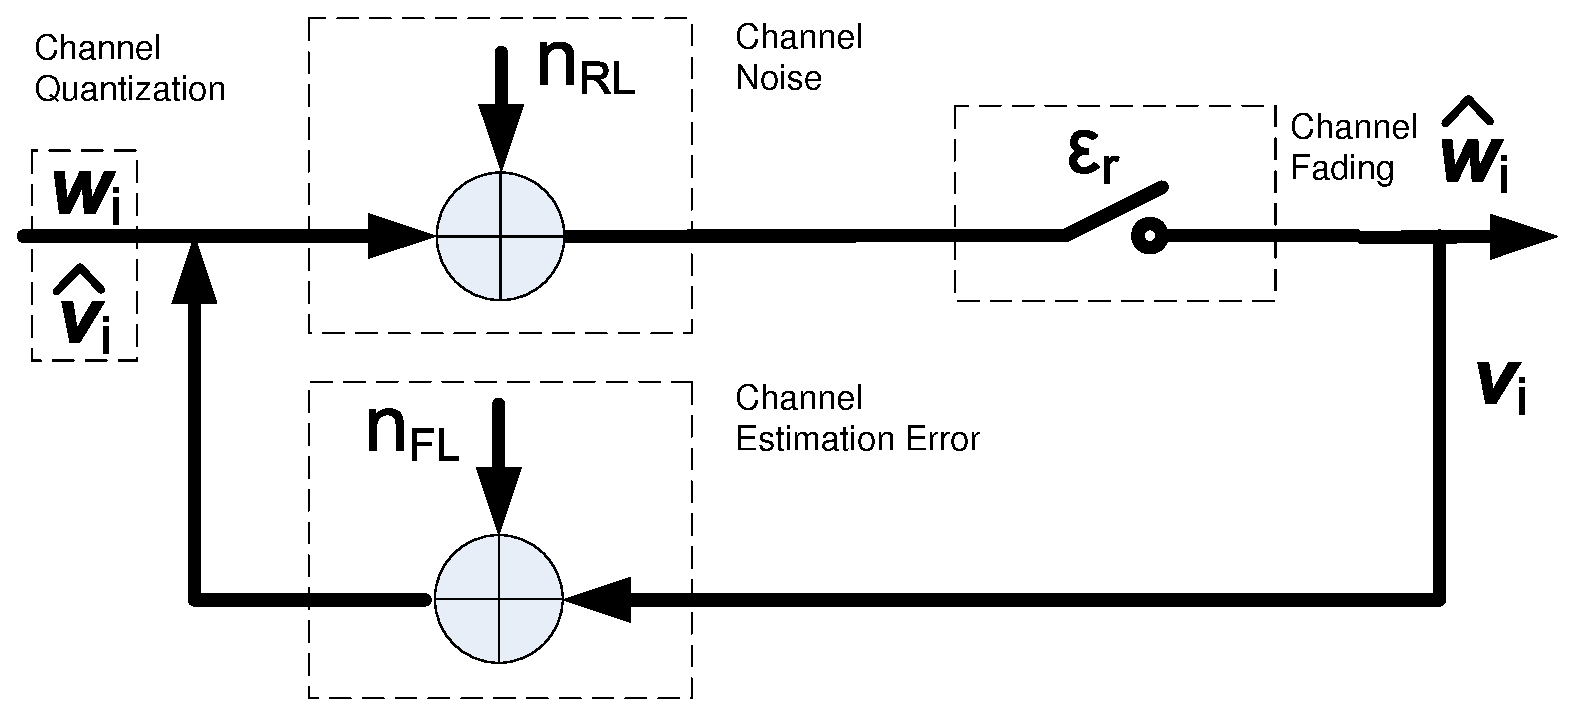
\includegraphics[width=3.0in, angle=0]{Noisy_Gaussian_Feedback_Channel3.eps}
\caption{Noisy Gaussian binary erasure feedback channel with
channel quantization.}\label{noisy_Gaussian_feedback} }
\end{figure}

MIMO beamforming with finite-rate feedback is modelled as a noisy
Gaussian binary erasure feedback channel depicted in
Fig.~\ref{noisy_Gaussian_feedback}. In reality, the receivers
estimate $\bH$ or $\bR_{\bH}$ with the pilots sent by transmitter.
Accuracy of the channel estimation depends on both forwardlink
design and receiver design. The pilot transmission is very helpful
for receiver to estimate CSI. After channel estimation, the
receiver chooses a beamforming vector from a shared MIMO precoding
codebook. This is called channel quantization. It means the
receiver actually feeds back the chosen precoding index(es) to
transmitter(s) instead of actual channel response for the next
transmitter precoding. With a MIMO codebook $\bcW$ of the size
$2^{R}$ consisting of $M$-dimensional normalized vectors
$\left\{\bw_{1}, ..., \bw_{2^{R}}\right\}$, it usually takes the
receiver to feedback $R$ bits for each beam stream. The codebook
is designed to quantize channel responses with certain distortion
measures~\cite{Narula98}. It is related to Grassmannian line
packing, the spherical packing on unit sphere
$\bcS_{n}\left(1\right)$~\cite{Love02} etc., where
$\bcS_{n}(r)=\left\{\bv:\ \left\|\bv\right\|=r\right\}$ denotes
$(n-1)$-sphere of radius $r$. When a codeword $\bw_k$ is chosen to
precode signals for $i$th beam $\bv_{i}$ at the transmitter side,
degradation will happen on the signals received by receiver
because of the imperfect channel estimation and finite-rate
feedback. The degradation on received signals can be expressed by
\begin{equation}
\begin{array}{rcl}
\delta_{i} & = & \min\limits_{\bw\in\bcW}\left\|\bH\bv_{i}-\bH\bw\right\|\\
&=&\lambda_{i}\left(1-\bv_{i}^{\rm
H}\bw_k\right)-\sum\limits_{j\neq i}\lambda_{j}\bv_{j}^{\rm
H}\bw_{k}
\end{array}\label{delta_i}
\end{equation}
\noindent where $\bv_{i}$ is the ideal precoding vector for $i$th
eigen-mode of $\bH$. It is known that $\delta_{i}$, which depends
on $\bv_{i}$, $\bw_{k}$ and $\lambda_{i}$, etc., is one of the
major factors limiting closed-loop MIMO beamforming throughput.
The reverselink channel is modelled by concatenating a Gaussian
channel and a binary erasure channel due to feedback redundancy
and the employed erasure mechanism, which drops those CSI packets
with low SNR.

In MIMO feedback channel design, the rate-distortion function and
the rate-reliability function are of the most important concerns.
For the rate-distortion function, the region of achievable rate
distortion pair $\left(R,\ D\right)$ with the squared error
distortion
\begin{equation}
\begin{array}{rcl}
D\left(R\right)&=&\max\limits_{i}\sum\limits_{m=1}^{M}\left(w_{i,m}-v_{i,m}\right)^2
\end{array}\label{squared_error_distortion}
\end{equation}
\noindent is of the most interests for understanding the effects
of channel estimation and quantization. On the other hand, the
achievable rate reliability pair $\left(R,\ \epsilon\right)$, with
the error exponent $\epsilon$ denoting how fast the reverselink
bit-error rate (BER) $P_{e}$ decays for the transmit rate $R$ and
given by

\begin{equation}
\begin{array}{rcccl}
\epsilon&=&\lim\limits_{n\rightarrow\infty}\sup
\epsilon_{n}&=&\lim\limits_{n\rightarrow\infty}\sup-\frac{1}{n}\ln
P_{e}
\end{array},
\end{equation}

\noindent where $\epsilon_{n}=-\frac{1}{n}\ln P_{e}$ denotes the
reliability of $n$-bits block transmission and $n$ is the minimum
block-length needed in order to operate at rate $R$ with the error
probability $P_{e}$, is of the most importance to understand the
performance of feedback design. In the following sections, we will
discuss how the imperfect channel estimation, quantization and
quality affect the achievable rate-distortion region and the
achievable rate-reliability region of MIMO feedback channel.

\section{The Rate-Distortion Region}

\subsection{Bemaforming Mismatch Lower Bound}
The channel quantization distortion is mostly decided by channel
quality, channel estimation algorithm and codebook design. In
general, the lower bound to the mean-squared error (MSE) of
unbiased channel estimates of $\bh$ is given by CRLB, which is
defined as the inverse of the Fisher Information Matrix (FIM),
\begin{equation}%\hspace{-0.10in}
\begin{array}{rcl}
\mbox{MSE}\left\{\bh-\hat{\bh}\right\}&\geq&\left[\bF\left(\vartheta\right)\right]^{-1}\\
&\hspace{-2.10in}=&\hspace{-1.10in}\mbox{E}^{-1}\left\{\left[\frac{\partial\ln\mbox{Pr}\left(\by|\vartheta\right)}{{\partial\vartheta}^{\ast}}\right]\left[\frac{\partial\ln\mbox{Pr}\left(\by|\vartheta\right)}{{\partial\vartheta}^{\ast}}\right]^{\rm
H}\right\}\end{array}\label{CRLB}
\end{equation}
\noindent with $\bvartheta$ the parameter vector to be estimated.
Given $\sigma_{\mbox{\tiny FL}}^{2}$ the MSE of forwardlink
channel estimation, the minimum rate at distortion $D_{\bh}$ is
given by
\begin{equation}\hspace{-0.20in}
\begin{array}{rcl}
R\left(D_{\bh}\right)&=&\min\limits_{E\|\bh-\hat{\bw}\|_{2}^{2}\leq
D_{\bh}} I\left(\bh_{i};\
\hat{\bh}_{i}\right)\\
&\hspace{-1.0in}=&\hspace{-0.50in}\min\limits_{E\|\bh_{i}-\hat{\bw}_{i}\|_{2}^{2}\leq
D_{\bh}}\left\{ H\left(\bh\right)-H\left(\bh|\hat{\bh}\right)\right\}\\
&\hspace{-1.0in}\geq&\hspace{-0.50in}M\log_{2}\left(2\pi
e\sigma_{\mbox{\tiny FL}}^{2}\right)-M\log_{2}\left(2\pi e
E\|h_{i}-\hat{w}_{i}\|_{2}^{2}\right)\\
&\hspace{-1.0in}=&\hspace{-0.50in}M\log_{2}\left(\frac{\sigma_{h}^{2}}{\frac{1}{M}D_{\bh}+\sigma_{\mbox{\tiny
FL}}^{2}}\right)
\end{array}\label{rate_distortion}
\end{equation}
\noindent with $0\leq\sigma_{h}^{2}\leq
\frac{1}{M}D_{\bh}+\sigma_{\mbox{\tiny FL}}^{2}$; otherwise,
$R\left(D_{\bh}\right)=0$. And the channel estimation error
$\sigma_{\mbox{\tiny FL}}$ is lower bounded by the CRLB in the
following lemma.

\begin{figure}
\center{
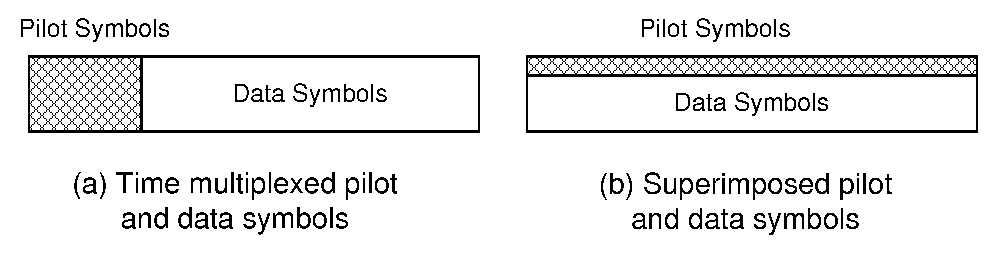
\includegraphics[width=3in, angle=0]{Pilot_Patterns.eps}
\caption{Pilot patterns for channel
estimation.}\label{pilot_pattern} }
\end{figure}

\begin{lemma}\label{Lemma_CRLB}(Cramer-Rao Lower Bound) For the time-multiplexed pilot and data design shown in Fig.~\ref{pilot_pattern}(a) and defined by
\begin{equation}
\begin{array}{rcl}
s_{k}\left(l\right)&=&
\begin{cases}
s_{pk}(l) & 1 \leq l \leq Q \\
s_{dk}(l-Q) & Q+1\leq l\leq L
\end{cases}
\end{array},\label{TMP_k}
\end{equation}
\noindent the CRLB of channel estimation is
\begin{equation}\hspace{-0.3in}
\begin{array}{rcccl}
\sigma_{\mbox{\tiny FL}}^{2}&\geq&\sigma_{\mbox{\tiny
TMP}}^{2}&=&\left[\rho_{h}^2+Q\rho_{p}^2+\left(L-Q\right)\rho_{d}^2\right]^{-1}
\end{array}.\label{CRLB_TMP}
\end{equation}
\noindent For the superimposed pilot and data design shown in
Fig.~\ref{pilot_pattern}(b) and defined by
\begin{equation}
\begin{array}{rcl}
s_{k}\left(l\right)&=&\frac{\sigma_{p}}{P}s_{pk}\left(l\right)+\frac{\sigma_{d}}{P}s_{dk}\left(l\right)\
,\ 1\leq l\leq L\ ,
\end{array}\label{SIP_k}
\end{equation}
\noindent with $\sigma_{p}^2+\sigma_{d}^2=P$, the CRLB of channel
estimation is
\begin{equation}\
\begin{array}{rcccl}
\sigma_{\mbox{\tiny FL}}^{2}&\geq&\sigma_{\mbox{\tiny
SIP}}^{2}&=&\left[\rho_{h}^2+L\left(\rho_{p}^2+\rho_{d}^2\right)\right]^{-1}
\end{array}\label{CRLB_SIP}
\end{equation}
\noindent where $\rho_{p}^2=\frac{\sigma_{p}^2}{\sigma_{n}^2}$
denotes the SNR of received pilot signals and
$\rho_{d}^2=\frac{\sigma_{d}^2}{\sigma_{n}^2}$ denotes the SNR of
received data signals.
\end{lemma}

(\ref{rate_distortion}) shows that the existence of channel
estimation error decreases the minimum codebook size necessitated
for channel quantization. When the channel estimation is very
"noisy" with $\sigma_{h}^{2}\leq\sigma_{\mbox{\tiny FL}}^{2}$, the
minimum codebook size is $R=0$
\begin{equation}%\hspace{-0.20in}
\begin{array}{rcl}
R\left(D\right)&\leq&0
\end{array},
\end{equation}
\noindent which means channel quantization may not be necessary
because of the bad channel estimation. When the channel estimation
is not so "noisy" but $\frac{M\sigma_{\mbox{\tiny
FL}}^{2}}{D_{\bh}}\gg 1$,
\begin{equation}%\hspace{-0.20in}
\begin{array}{rcl}
R(D_{\bh})&\gtrsim&M\log_{2}\left(\frac{\sigma_{h}^{2}}{\sigma_{\mbox{\tiny
FL}}^{2}}\right)\ .
\end{array}
\end{equation}
\noindent This means a too fine quantization may is unnecessary
since channel estimation error is dominant. Even with a good
estimation $\frac{M\sigma_{\mbox{\tiny FL}}^{2}}{D_{\bh}}\ll 1$,
it still requires that $D_{\bh}$ the channel quantization error
should be less than $M\left(\sigma_{h}^{2}-\sigma_{\mbox{\tiny
FL}}^{2}\right)$ the channel response deviation. Therefore, for
better performance, $D_{\bh}$ shall satisfies
\begin{equation}%\hspace{-0.20in}
\begin{array}{rcccl}
M\sigma_{\mbox{\tiny
FL}}^{2}&\ll&D_{\bh}&\leq&M\left(\sigma_{h}^{2}-\sigma_{\mbox{\tiny
FL}}^{2}\right)\ .
\end{array}
\end{equation}
\noindent When $D_{\bh}$ is proper and the role of channel
quantization becomes important, the squared error rate distortion
$D_{\bh}$ can be written by
\begin{equation}%\hspace{-0.20in}
\begin{array}{rcl}
D_{\bh}&=&\max\limits_{i}\left\|\bh_{i}-w_{r}{\bw}_{\phi}\right\|_{2}^{2}
\end{array}\label{D_h}
\end{equation}
\noindent with $w_{r}$ denoting the quantized vector channel norm
and ${\bw}_{\phi}$ denoting the quantized vector channel phase. In
existing MIMO beamforming system design, the receiver usually
tracks the channel norm information for adaptive modulation
purpose and phase quantization instead of quantizing and feeding
back the channel norm. In this case, (\ref{D_h}) can be rewritten
by
\begin{equation}\hspace{-0.10in}
\begin{array}{rcl}
D_{\bh}&=&\max\limits_{i}\mbox{E}\left\|\bh_{i}-\hat{r}{\bw}_{\phi}\right\|_{2}^{2}\\
&=&\max\limits_{i}\left\{\mbox{E}\left\|r\left(\bv_{i}-{\bw}_{\phi}\right)\right\|_{2}^{2}+\mbox{E}\left\|\delta_{r}{\bw}_{\phi}\right\|_{2}^{2}\right\}\\
&=&2M\sigma_{h}^{2}\left(1-\sqrt{1-D_{\phi}}\right)+\sigma_{\mbox{\tiny
FL}}^{2}\ .
\end{array}\label{D_h2}
\end{equation}
\noindent with $\hat{r}$ denoting the estimate of the channel norm
$r$ and $D_{\phi}=\mbox{var}\left\{\sin\angle\left(\bv,\
\bw\right)\right\}$ denoting the phase quantization deviation.
Therefore a lower bound for distortion rate of channel
quantization for MIMO beamforming is
\begin{equation}%\hspace{-0.10in}
\begin{array}{rcl}
R(D_{\phi})&=&\min\limits_{E\|\bv_{i}-\hat{\bv}_{i}\|_{2}^{2}\leq
D_{\phi}} I\left(\bv_{i};\
\hat{\bv}_{i}\right)\\
&\geq&M\log_{2}\left(\frac{\sigma_{h}^{2}}{\frac{M+1}{M}\sigma_{\mbox{\tiny
FL}}^{2}+\sigma_{h}^{2}\left(1-D_{\phi}\right)}\right)\ .
\end{array}\label{R_D_phi}
\end{equation}
\noindent for each beam. With the feedback rate of $R$,
(\ref{R_D_phi}) also tells us that the minimum precoding mismatch
for forwardlink MIMO beamforming is
\begin{equation}%\hspace{-0.10in}
\begin{array}{rcl}
D_{\phi}&=&\max\mbox{E}\left\{1-\left\|\hat{\bv}-\bv\right\|_{2}^{2}\right\}\\
 &\leq&1-2^{-\frac{R}{M}}+\frac{M+1}{M}\frac{\sigma_{\mbox{\tiny
FL}}^{2}}{\sigma_{h}^{2}}\ .
\end{array}\label{D_phi}
\end{equation}

\subsection{Bemaforming Mismatch Upper Bound}
\begin{figure}
\center{
\includegraphics[width=3.20in, angle=0]{Voronoi_Bounds2.eps}
\caption{Voronoi cell and various bounds}\label{Voronoi_bound} }
\end{figure}
The beamforming mismatch upper bound depends on the codebook
design. The maximum beamforming mismatch can be determined by the
largest radius of the codebook Voronoi cell $\left\{\bcV_{i}:\
1\leq i\leq 2^{R}\right\}$, which in general is the solution to
the disk-covering problem that still is open. Instead of the exact
boundary for the Voronoi cell $\bcV_{i}$, we suggest a heuristic
approach using sphere-packing bound and sphere cap to approximate
the actual polytope boundary. It is an approximate of the sphere
packing solution, in which all spheres are supposed to be
non-overlappedly placed. With our approach, sphere caps are
overlapped with each other in space but the interior of them has
the same area as the Voronoi cell. The border of this sphere cap
is termed sphere-packing boundary. The relationship between
sphere-packing boundary and Voronoi cell is shown in
Fig.~\ref{Voronoi_bound}. For an uniform random codebook of size
$2^{R}$ in $M$-dimensional Euclid space, the area of a Voronoi
cell is given by
\begin{equation}
\begin{array}{rcl}
A\left(\bcV_{k}\right)&=&
\frac{2{\pi}^{M}}{2^{R}\Gamma\left(M\right)}
\end{array}\label{V_area}
\end{equation}
\noindent where $\Gamma\left(\ast\right)$ denotes the gamma
function. On the other hand, the area of $(m-1)$-complex sphere
cap $\bcC_{m}^{\rm c}\left(\psi,\ R\right)$ with contact angle
$\psi$ and radius $r$ is
\begin{equation}%\hspace{-0.22in}
\begin{array}{l}
A\left(\bcC_{m}^{\rm c}\left(\psi,\
r\right)\right)=\left[1-\cos^{2(m-1)}\left(\psi\right)\right]S_{m}^{\rm
c}\left(r\right),
\end{array}
\end{equation}
\noindent where ${\bcS}_{m}^{\rm c}\left(r\right)$ denotes a
$M$-dimension complex ball in Euclid space with the radius $r$.
The relationship between ${\bcS}_{m}^{\rm c}\left(r\right)$ and
$\bcC_{m}^{\rm c}\left(\psi,\ r\right)$ can be shown in
Fig.~\ref{Voronoi_bound} and it can be verified that
\begin{equation}
\begin{array}{rcl}
A\left(S_{m}^{c}\left(r\right)\right)&=&A\left(\bcC_{m}^{\rm
c}\left(\pi,\ r\right)\right)
\end{array}.
\end{equation}
\noindent With matching the sum area of the sphere-cap with the
whole sphere area, the boundary of a Voronoi cell can be
approximated by a hypershpere or a closed space curve defined in
the following proposition.
\begin{lemma}\label{approx_bound}(Sphere-packing Boundary) The boundary of the uniform complex Voronoi cell $\bcV_{k}$ can be
approximated by a $(M-1)$-unit complex sphere or a closed complex
space curve.
\begin{equation}\hspace{-0.05in}
\begin{array}{rcl}
\bB\left(\bcV_{k}\right)&\approx& \bcS_{M}^{\rm c}(1)\bigcap \bcL_{M}^{\rm c}(\bw_{k},\ \cos(\theta)) \\
&=&\left\{\bv:\ \left\|\bv\right\|=1,\ \angle\left(\bv,\
\bw_{k}\right)=\theta\right\}\ ,
\end{array}
\end{equation}
\noindent where $\bcL_{M}^{\rm c}\left(\bw_{k},\
\cos(\theta)\right)=\left\{\bv:\ \bv^{\rm
H}\bw_{k}=\cos(\theta)\right\}$ denotes a complex space curve and
$\theta$ is
\begin{equation}%\hspace{-0.00in}
\begin{array}{rcl}
\theta&=&\arccos\left(\alpha_{0}\right)
\end{array}
\end{equation}
\noindent with
\begin{equation}\hspace{-0.00in}
\begin{array}{rcl}
\alpha_{0}&=&\left(\frac{2^{R}-1}{2^R}\right)^{\frac{1}{2M-2}}
\end{array}.
\end{equation}
\end{lemma}
With Lemma \ref{approx_bound}, a heuristic upper bound of MIMO
beamforming mismatch is given by

\begin{equation}
\begin{array}{rcl}
D_{\phi}&\leq&\left[1-\left(\frac{2^{R}-1}{2^R}\right)^{\frac{1}{M-1}}\right]^{\frac{1}{2}}
\end{array}.\label{distortion_upper_bound}
\end{equation}
\noindent With (\ref{D_phi}) and (\ref{distortion_upper_bound}),
the rate-distortion region can be written by
\begin{equation}\hspace{-0.10in}
\begin{array}{l}
2^{-\frac{R}{M}}-\left(1+\frac{1}{M}\right)\frac{\sigma_{\mbox{\tiny
FL}}^{2}}{\sigma_{h}^{2}}\ \leq\ D_{\phi}\ \leq\
\left[1-\left(\frac{2^{R}-1}{2^R}\right)^{\frac{1}{M-1}}\right]^{\frac{1}{2}}.
\end{array}
\end{equation}
\noindent One example of the rate-distortion region is shown in
Fig.~\ref{Rate_Distortion}.
\begin{figure}
\center{
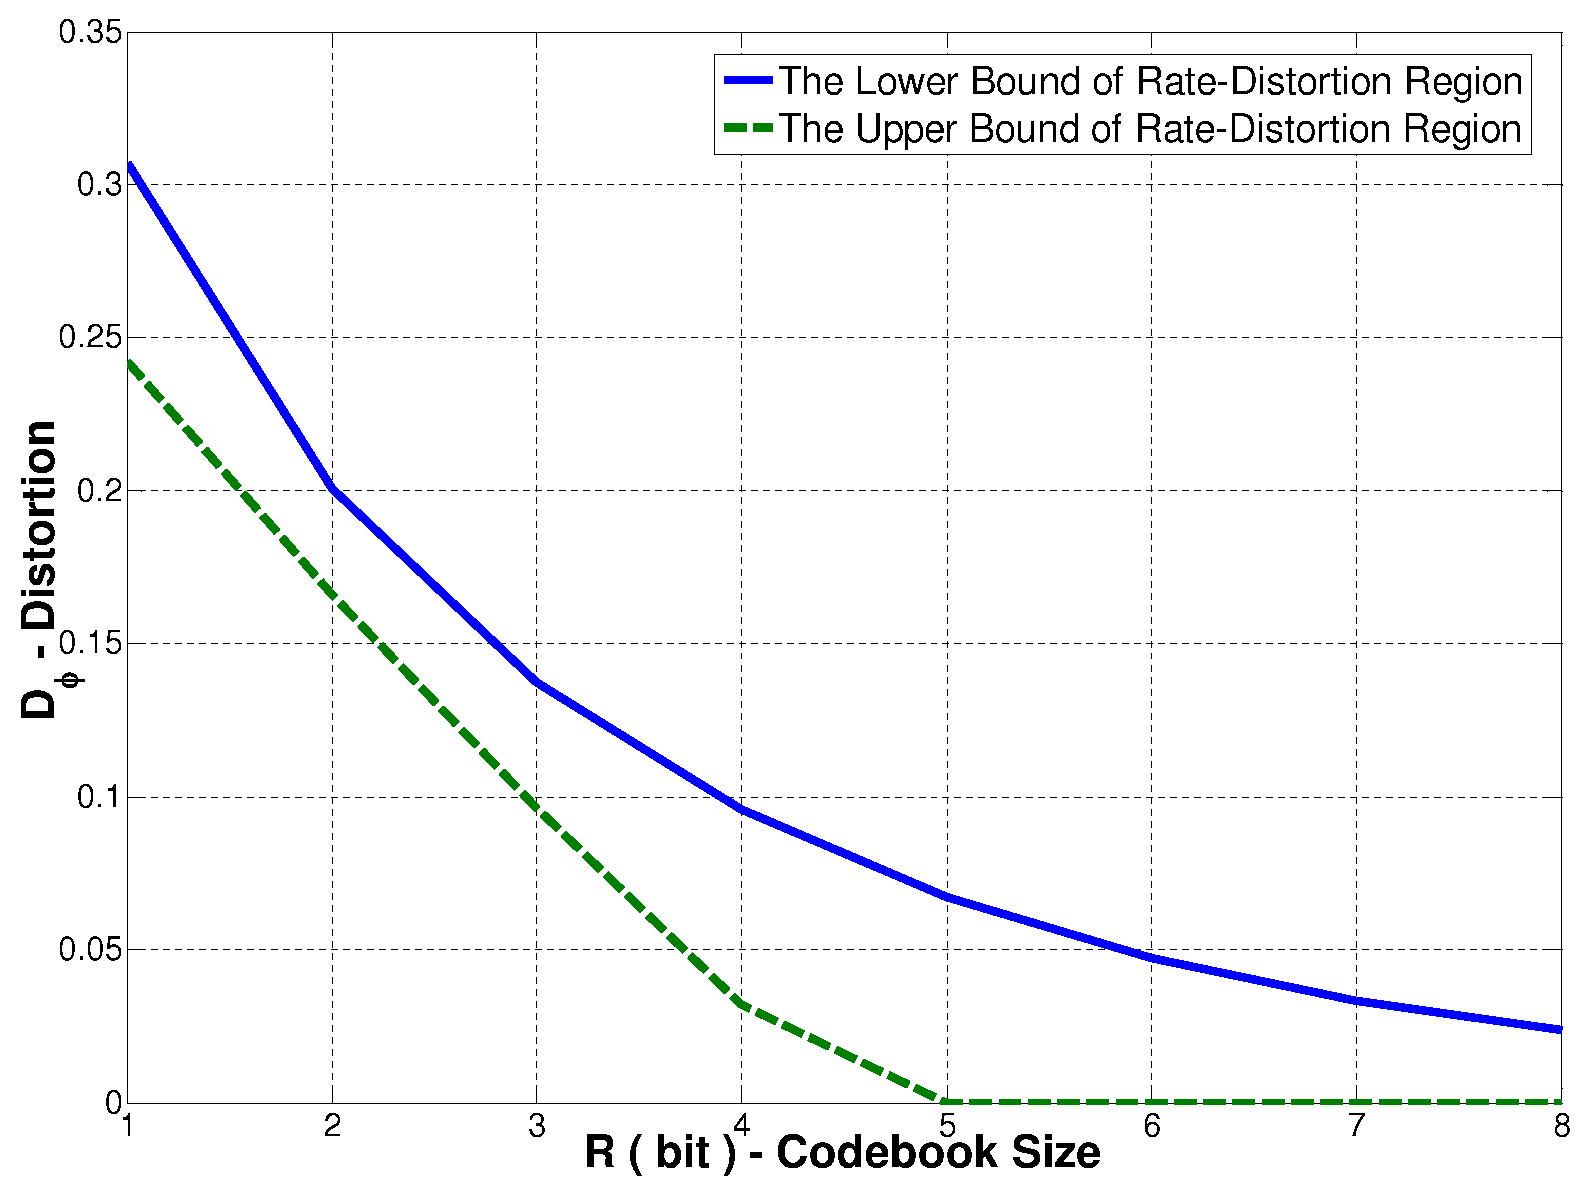
\includegraphics[width=3.20in, angle=0]{Rate_Distortion.eps}
\caption{The rate-distortion region with $M=8$ and
$\frac{\sigma_{h}^{2}}{\sigma_{\mbox{\tiny
FL}}^{2}}=2.2$dB.}\label{Rate_Distortion} }
\end{figure}


\section{The Rate-Reliability Region}

The reverselink channel model is a concatenation of a Gaussian
channel and binary erasure channel, which are independent to each
other. In generally, the reliability of reverselink is controlled
by both channel fading and received SNR. When the erasure rate
$\varepsilon_{r}$ is high, it means the amount of fading of
reverselink is very high. Higher erasure rate also means it takes
the forwardlink transmitter longer time to accurately filter out a
proper forwardlink precoding word and it usually yields higher
MIMO precoding mismatch given a certain channel coherent time.
Since the unreliable symbols are erased based on their received
SNR, the left symbols are more reliable and their reliability is
mostly decided by $\gamma_{\mbox{\tiny RL}}$. In this case, the
well-known sphere-packing upper bound of Gaussian channel
reliability function is
\begin{equation}%\hspace{-0.00in}
\begin{array}{rcl}
\epsilon\left(R\right)&\leq&\epsilon_{\rm sp}\left(R\right)
\end{array}\label{reliability_upper_bound}
\end{equation}
\noindent with $\epsilon_{\rm
sp}\left(R\right)=\frac{\gamma_{\mbox{\tiny
RL}}}{2}-\frac{\sqrt{\gamma_{\mbox{\tiny
RL}}}\eta\cos\theta}{2}-\ln\left(\eta\sin\theta\right)$ and the
lower bound is
\begin{equation}\hspace{-0.30in}
\begin{array}{l}
\epsilon\left(R\right)\geq\begin{cases} \frac{\gamma_{\mbox{\tiny
RL}}}{4}\left(1-\cos\theta\right) &
0\leq R\leq R_{1} \\
\frac{\gamma_{\mbox{\tiny RL}}}{4}\left(1-\cos\theta_{1}\right)
+R_{1}-R&
R_{1}\leq R\leq R_{2} \\
\epsilon_{\rm sp}\left(R\right) &R_{2}\leq R\leq C
\end{cases}
\end{array}\label{reliability_lower_bound}
\end{equation}
\noindent where $\gamma_{\mbox{\tiny RL}}=\frac{P_{\mbox{\tiny
RL}}}{\sigma^2_{\mbox{\tiny RL}}}$ denotes the reverselink SNR,
$\theta=\arcsin e^{-R}$ denotes the sphere-packing angle,
\begin{equation}\hspace{-0.0in}
\begin{array}{rcl}
\eta&=&\frac{1}{2}\left(\sqrt{\gamma_{\mbox{\tiny
RL}}}\cos\theta+\sqrt{\gamma_{\mbox{\tiny
RL}}\cos^2\theta+4}\right)
\end{array},
\end{equation}
\begin{equation}\hspace{-0.0in}
\begin{array}{rcl}
R_{1}&=&\frac{1}{2}\ln\left(\frac{1}{2}+\frac{1}{2}\sqrt{1+\frac{\gamma_{\mbox{\tiny
RL}}}{4}}\right)
\end{array},
\end{equation}
\begin{equation}\hspace{-0.0in}
\begin{array}{rcl}
R_{2}&=&\frac{1}{2}\ln\left(\frac{1}{2}+\frac{\gamma_{\mbox{\tiny
RL}}}{4}+\frac{1}{2}\sqrt{1+\frac{\gamma_{\mbox{\tiny
RL}}}{4}}\right)
\end{array}
\end{equation}
\noindent and $\theta_{1}=\arcsin e^{-R_{1}}$. The
rate-reliability region with sphere-packing bounds is shown in
Fig.~\ref{Rate_Reliability}.

\begin{figure}
\center{
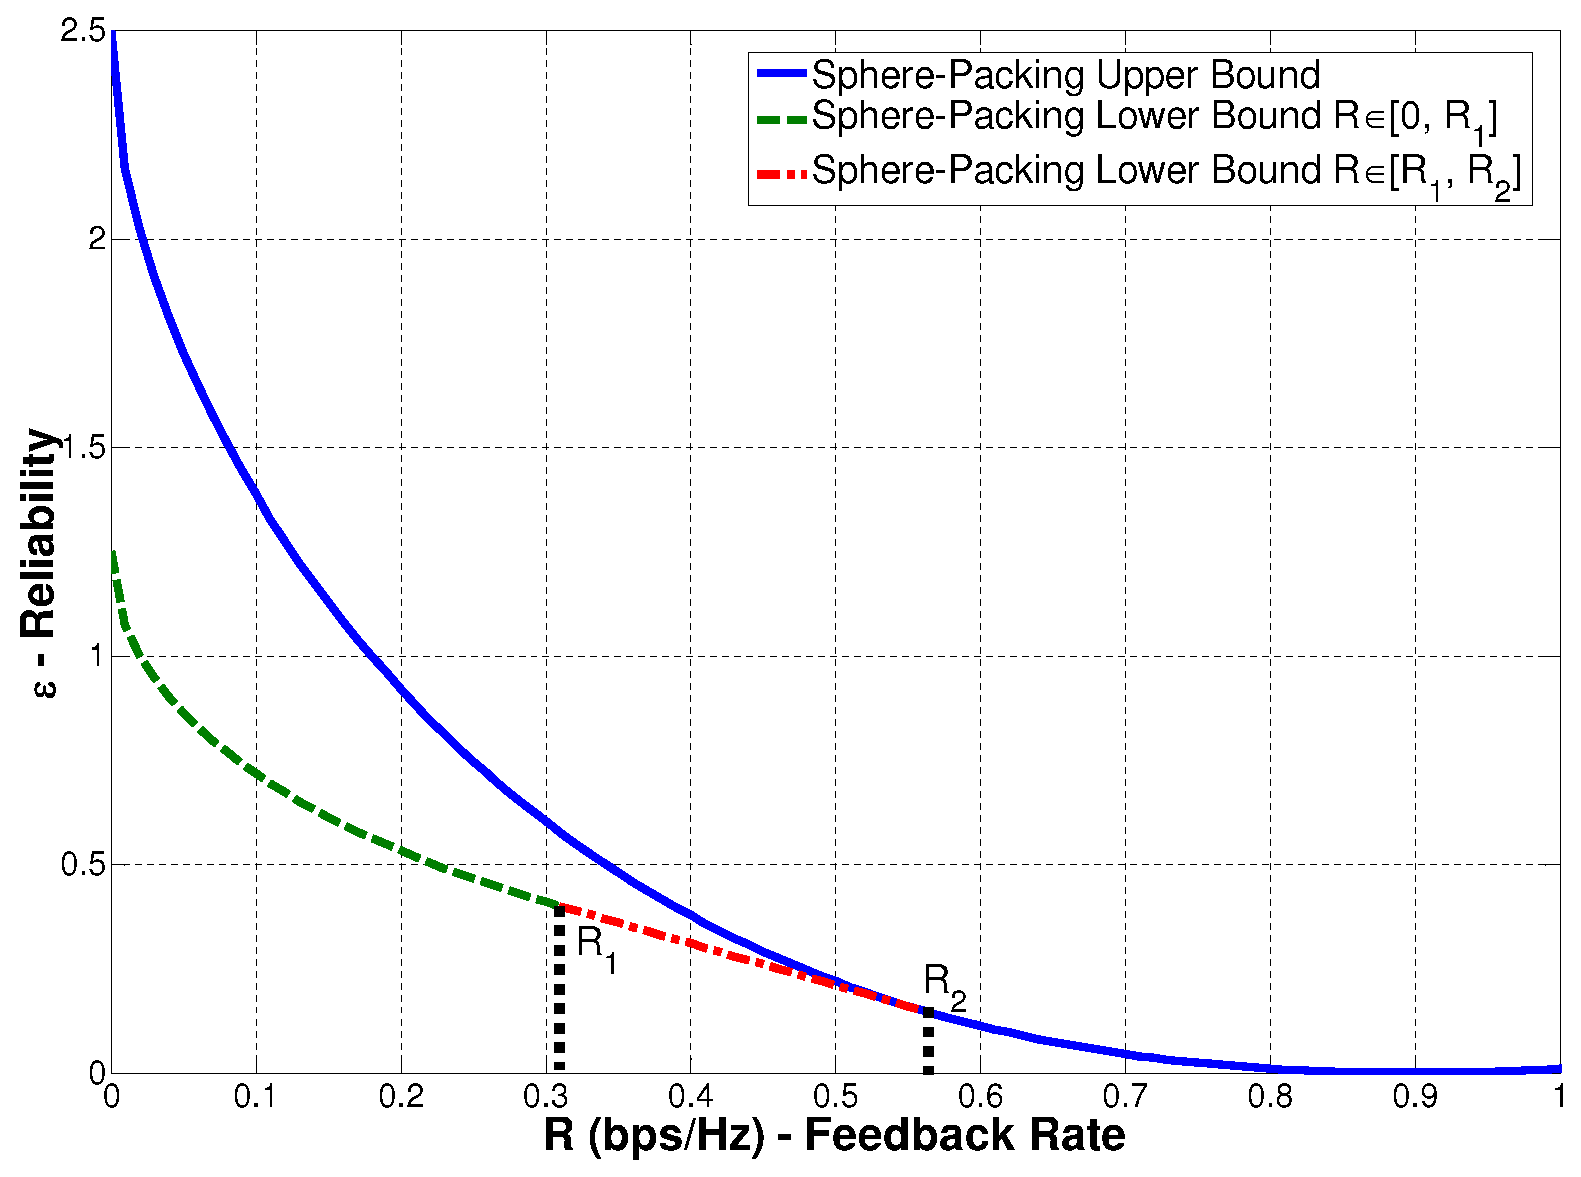
\includegraphics[width=3.20in, angle=0]{Rate_Reliability2.eps}
\caption{The rate-reliability region with ${\gamma_{\mbox{\tiny
RL}}}=7$dB.}\label{Rate_Reliability} }
\end{figure}

\section{Conclusions}
In this paper, the distortion and reliability of MIMO beamforming
feedback channel, which is modelled as a Gaussian binary erasure
channel, are discussed for the problem how much feedback is
necessary. The lower bound and upper bound for the rate-distortion
region and the rate-reliability region of MIMO beamforming
feedback are therefore derived. The tradeoffs between codebook
design and channel structure are revealed.

\small
\bibliographystyle{unsrt}
\bibliography{Cooperative_Relay}
\end{document}
